%%%%%%%%%%%%%%%%%%%%%%%%%%%%%%%%%%%%%%%%%%%%%%%%%%%%%%%%%%%%%%%%%%%%%%
% Overleaf (WriteLaTeX) Example: Molecular Chemistry Presentation
%
% Source: http://www.overleaf.com
%
% In these slides we show how Overleaf can be used with standard 
% chemistry packages to easily create professional presentations.
% 
% Feel free to distribute this example, but please keep the referral
% to overleaf.com
% 
%%%%%%%%%%%%%%%%%%%%%%%%%%%%%%%%%%%%%%%%%%%%%%%%%%%%%%%%%%%%%%%%%%%%%%

\documentclass{beamer}

\mode<presentation>
{
  \usetheme{Madrid}       % or try default, Darmstadt, Warsaw, ...
  \usecolortheme{default} % or try albatross, beaver, crane, ...
  \usefonttheme{default}    % or try default, structurebold, ...
  \setbeamertemplate{navigation symbols}{}
  \setbeamertemplate{caption}[numbered]
} 

\usepackage[english]{babel}
\usepackage[utf8x]{inputenc}
\usepackage{chemfig}
\usepackage[version=3]{mhchem}

\usepackage{hyperref}
  \hypersetup{colorlinks=true}
  \hypersetup{urlcolor=blue}
  \hypersetup{linkcolor = .}
\usepackage{xcolor}
\usepackage{siunitx}
  \sisetup{separate-uncertainty = true}
\usepackage{physics}
\usepackage[font=small,labelfont=bf]{caption}
\usepackage{subcaption}
\usepackage[en-GB]{datetime2}
\usepackage{feynmp}
\DeclareGraphicsRule{*}{mps}{*}{}

\usepackage{scalerel}
\newcommand{\mylbrace}[2]{\vspace{#2pt}\hspace{6pt}\scaleleftright[\dimexpr5pt+#1\dimexpr0.06pt]{\lbrace}{\rule[\dimexpr2pt-#1\dimexpr0.5pt]{-4pt}{#1pt}}{.}}
\newcommand{\myrbrace}[2]{\vspace{#2pt}\scaleleftright[\dimexpr5pt+#1\dimexpr0.06pt]{.}{\rule[\dimexpr2pt-#1\dimexpr0.5pt]{-4pt}{#1pt}}{\rbrace}\hspace{6pt}}

% Here's where the presentation starts, with the info for the title slide
\title[LHCb UK Annual Meeting]{LHCb UK Annual Meeting}
\author{Martin Tat}
\institute{Oxford LHCb}
\date{8th January 2021}

\titlegraphic{
\includegraphics[width = 5cm, height = 3.8cm]{lhcb.jpg}\hspace{1cm}~%
              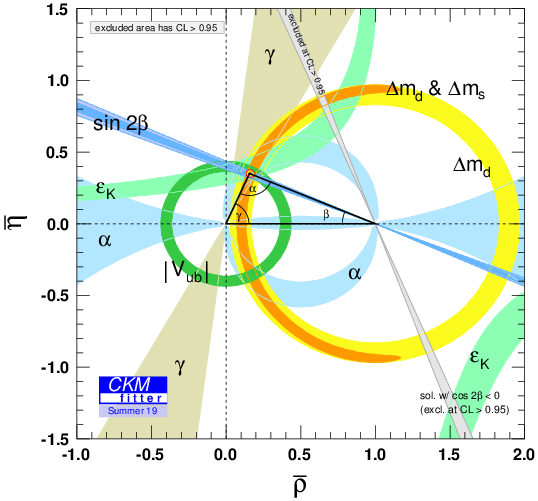
\includegraphics[width = 5cm, height = 3.8cm]{ckmfitter.png}}

\begin{document}

\begin{frame}
  \titlepage
\end{frame}

% These three lines create an automatically generated table of contents.
%\begin{frame}{Outline}
%  \tableofcontents
%\end{frame}

\section{Myself}
\begin{frame}{About myself}
  \begin{itemize}
    \item{From Kristiansand, Norway}
    \item{4-year Master of Physics, University of Oxford}
    \item{PhD with LHCb at University of Oxford}
    \item{Supervisors:}
    \begin{itemize}
      \item{Prof Guy Wilkinson (analysis)}
      \item{Prof Neville Harnew (detector)}
    \end{itemize}
  \end{itemize}
\end{frame}

\section{My project}
\begin{frame}{Analysis project: $\gamma$ measurement}
  \begin{itemize}
    \item{$B^\pm\to DK^\pm, \quad D = D^0,\bar{D^0}$}
    \begin{itemize}
      \item{$D\to K^+K^-\pi^+\pi^-$}
    \end{itemize}
    \item{Interference between $b\to c$ and $b\to u$ $\implies\gamma$ measurement!}
    \item{$4$-body decay $\implies 5$-dimensional phase space}
    \item{Strong phase inputs from BESIII}
  \end{itemize}
  \begin{figure}[H]
    \centering
    \vspace{0.3cm}
    \begin{subfigure}{0.5\textwidth}
      \centering
      \begin{fmffile}{fgraph_BtoDK1}
        \setlength{\unitlength}{0.4cm}
        \begin{fmfgraph*}(6,6)
          \fmfstraight
          \fmfleft{i1,B,i2,t1,t2,t3,t9,t10}
          \fmfright{o1,D,o2,t4,t5,o3,K,o4}
          \fmflabel{$\bar{u}$}{i1}
          \fmflabel{$b$}{i2}
          \fmfv{l.d=20,l.a=180,l={$B^-$\mylbrace{30}{-8}}}{B}
          \fmflabel{$\bar{u}$}{o1}
          \fmflabel{$c$}{o2}
          \fmflabel{$\bar{u}$}{o3}
          \fmflabel{$s$}{o4}
          \fmfv{l.d=15,l.a=0,l={\myrbrace{30}{-12}}$D^0$}{D}
          \fmfv{l.d=15,l.a=0,l={\myrbrace{30}{11}}$K^-$}{K}
          \fmf{fermion}{o1,i1}
          \fmf{fermion,tension=1.5}{i2,v1}
          \fmf{fermion}{v1,o2}
          \fmf{phantom,tension=1.5}{t9,v2}
          \fmf{boson,label=$W$,label.side=left,tension=0}{v1,v2}
          \fmf{fermion}{v2,o4}
          \fmf{fermion}{o3,v2}
        \end{fmfgraph*}
      \end{fmffile}
      \vspace{0.5cm}
      \caption{$B^-\to D^0K^-$}
    \end{subfigure}%
    \begin{subfigure}{0.5\textwidth}
      \centering
      \begin{fmffile}{fgraph_BtoDK2}
        \setlength{\unitlength}{0.4cm}
        \begin{fmfgraph*}(6,6)
          \fmfstraight
          \fmfleft{i1,t1,t2,B,t9,t10,i2}
          \fmfright{o1,K,o2,t4,t5,o3,D,o4}
          \fmflabel{$\bar{u}$}{i1}
          \fmflabel{$b$}{i2}
          \fmfv{l.d=20,l.a=180,l={$B^-$\mylbrace{100}{-8}}}{B}
          \fmflabel{$\bar{u}$}{o1}
          \fmflabel{$s$}{o2}
          \fmflabel{$\bar{c}$}{o3}
          \fmflabel{$u$}{o4}
          \fmfv{l.d=15,l.a=0,l={\myrbrace{30}{13}}$\bar{D^0}$}{D}
          \fmfv{l.d=15,l.a=0,l={\myrbrace{30}{-13}}$K^-$}{K}
          \fmf{fermion}{o1,i1}
          \fmf{fermion,tension=1.5}{i2,v1}
          \fmf{fermion}{v1,o4}
          \fmf{phantom,tension=1.5}{t2,v2}
          \fmf{boson,label=$W$,label.side=left,tension=0}{v1,v2}
          \fmf{fermion}{v2,o2}
          \fmf{fermion}{o3,v2}
        \end{fmfgraph*}
      \end{fmffile}
      \vspace{0.5cm}
      \caption{$B^-\to\bar{D^0}K^-$}
    \end{subfigure}
  \end{figure}
\end{frame}

\begin{frame}{Analysis project: $\gamma$ measurement}
  \begin{itemize}
    \item{Unbinned model-dependent fit}
    \begin{itemize}
      \item{LHCb isobar amplitude model \href{https://arxiv.org/abs/1811.08304}{arXiv:1811.08304}}
      \item{Generate events and fit to the same model}
      \item{$\gamma$ precision: $11^\circ$ with $2000$ events}
    \end{itemize}
    \item{Binned model-independent fit}
    \begin{itemize}
      \item{Develop binning scheme}
      \item{$\gamma$ precision with $8$ bins: $13^\circ$, $12^\circ$ with further modifications}
      \item{$\gamma$ precision with $4$ bins: $15^\circ$, $14^\circ$ with further modifications}
    \end{itemize}
    \item{Next steps:}
    \begin{itemize}
      \item{Pick out events from LHCb and BESIII data}
      \item{Extract strong phases from BESIII data and measure $\gamma$ from LHCb data}
      \item{TORCH with Prof Neville Harnew}
    \end{itemize}
  \end{itemize}
\end{frame}

\end{document}
